\documentclass[]{article}
\usepackage{lmodern}
\usepackage{amssymb,amsmath}
\usepackage{ifxetex,ifluatex}
\usepackage{fixltx2e} % provides \textsubscript
\ifnum 0\ifxetex 1\fi\ifluatex 1\fi=0 % if pdftex
  \usepackage[T1]{fontenc}
  \usepackage[utf8]{inputenc}
\else % if luatex or xelatex
  \ifxetex
    \usepackage{mathspec}
  \else
    \usepackage{fontspec}
  \fi
  \defaultfontfeatures{Ligatures=TeX,Scale=MatchLowercase}
\fi
% use upquote if available, for straight quotes in verbatim environments
\IfFileExists{upquote.sty}{\usepackage{upquote}}{}
% use microtype if available
\IfFileExists{microtype.sty}{%
\usepackage{microtype}
\UseMicrotypeSet[protrusion]{basicmath} % disable protrusion for tt fonts
}{}
\usepackage[margin=1in]{geometry}
\usepackage{hyperref}
\hypersetup{unicode=true,
            pdftitle={A gene-diet interaction-based score predicts response to dietary fat in the Women's Health Initiative},
            pdfborder={0 0 0},
            breaklinks=true}
\urlstyle{same}  % don't use monospace font for urls
\usepackage{graphicx,grffile}
\makeatletter
\def\maxwidth{\ifdim\Gin@nat@width>\linewidth\linewidth\else\Gin@nat@width\fi}
\def\maxheight{\ifdim\Gin@nat@height>\textheight\textheight\else\Gin@nat@height\fi}
\makeatother
% Scale images if necessary, so that they will not overflow the page
% margins by default, and it is still possible to overwrite the defaults
% using explicit options in \includegraphics[width, height, ...]{}
\setkeys{Gin}{width=\maxwidth,height=\maxheight,keepaspectratio}
\IfFileExists{parskip.sty}{%
\usepackage{parskip}
}{% else
\setlength{\parindent}{0pt}
\setlength{\parskip}{6pt plus 2pt minus 1pt}
}
\setlength{\emergencystretch}{3em}  % prevent overfull lines
\providecommand{\tightlist}{%
  \setlength{\itemsep}{0pt}\setlength{\parskip}{0pt}}
\setcounter{secnumdepth}{0}
% Redefines (sub)paragraphs to behave more like sections
\ifx\paragraph\undefined\else
\let\oldparagraph\paragraph
\renewcommand{\paragraph}[1]{\oldparagraph{#1}\mbox{}}
\fi
\ifx\subparagraph\undefined\else
\let\oldsubparagraph\subparagraph
\renewcommand{\subparagraph}[1]{\oldsubparagraph{#1}\mbox{}}
\fi

%%% Use protect on footnotes to avoid problems with footnotes in titles
\let\rmarkdownfootnote\footnote%
\def\footnote{\protect\rmarkdownfootnote}

%%% Change title format to be more compact
\usepackage{titling}

% Create subtitle command for use in maketitle
\providecommand{\subtitle}[1]{
  \posttitle{
    \begin{center}\large#1\end{center}
    }
}

\setlength{\droptitle}{-2em}

  \title{A gene-diet interaction-based score predicts response to dietary fat in
the Women's Health Initiative}
    \pretitle{\vspace{\droptitle}\centering\huge}
  \posttitle{\par}
    \author{}
    \preauthor{}\postauthor{}
    \date{}
    \predate{}\postdate{}
  
\usepackage{booktabs}
\usepackage{longtable}
\usepackage{array}
\usepackage{multirow}
\usepackage{wrapfig}
\usepackage{float}
\usepackage{colortbl}
\usepackage{pdflscape}
\usepackage{tabu}
\usepackage{threeparttable}
\usepackage{threeparttablex}
\usepackage[normalem]{ulem}
\usepackage{makecell}
\usepackage{xcolor}

\begin{document}
\maketitle

\hypertarget{abstract}{%
\section{Abstract}\label{abstract}}

\textbf{Background:} While diet response prediction for cardiometabolic
risk factors (CRFs) has been demonstrated using single genetic variants
and main-effect genetic risk scores, little investigation has gone into
the development of genome-wide diet response scores.

\textbf{Objective:} Here, we sought to leverage the multi-study setup of
the Women's Health Initiative cohort to generate and test genetic scores
for the response of six CRFs (body mass index, systolic blood pressure,
LDL-cholesterol, HDL-cholesterol, triglycerides, and fasting glucose) to
dietary fat.

\textbf{Design:} A genome-wide interaction study was undertaken for each
CRF in women (n \textasciitilde{} 9000) not participating in the Dietary
Modification (DM) trial, which focused on the reduction of dietary fat.
Genetic scores based on these analyses were developed using a
pruning-and-thresholding approach and tested for the prediction of
one-year CRF changes as well as long-term chronic disease development in
DM trial participants (n \textasciitilde{} 5000).

\textbf{Results:} Only one of these genetic scores, for LDL-cholesterol
(LDL-C), predicted changes in the associated CRF. This 1760-variant
score explained 3.7\% (95\% CI: 0.09, 11.9) of the variance in one-year
LDL-C changes in the intervention arm, but was unassociated with changes
in the control arm. In contrast, a main-effect genetic risk score for
LDL-C was not useful for predicting dietary fat response. Further
investigation of this score with respect to downstream disease outcomes
revealed suggestive differential associations across DM trial arms,
especially with respect to coronary heart disease and stroke subtypes.

\textbf{Conclusions:} These results lay the foundation for the
combination of many genome-wide gene-diet interactions for diet response
prediction while highlighting the need for further research and larger
samples in order to achieve robust biomarkers for use in personalized
nutrition.

\hypertarget{introduction}{%
\section{Introduction}\label{introduction}}

Nutrigenetics approaches, in which genetic information is used to
predict response to dietary inputs, are central to the emerging promise
of personalized nutrition for cardiometabolic risk reduction.
Inter-individual differences in food preferences, metabolism,
detoxification, excretion, etc. affect our responses to diet, in a
similar manner to the well-studied field of pharmacogenomics (1).
Ideally, genotype-based nutrigenetic investigations would be conducted
in large-scale dietary interventions. Two notable examples are the
PREDIMED and POUNDS LOST trial, with significant findings including the
interaction of a \emph{TCF7L2} variant with a Mediterranean diet pattern
for glycemic traits (2) and the interaction of a \emph{PCSK9} variant
with dietary carbohydrate for insulin resistance (3). However, such
intervention-based studies are able to examine only a single dietary
change (whether food, nutrient, or pattern) at a time, and are often
limited to lower sample sizes (4).

To allow for more flexibility and greater sample sizes, gene-diet
interactions (GDIs) are more commonly investigated in observational
datasets. There is a rich literature of GDI discovery in the
cardiometabolic realm. Typically, these focus on cardiometabolic risk
factors in relation to biology-based candidate genes/variants (5,6), but
some have looked at clinical outcomes (e.g.~MI (7)). Other approaches
use main-effect genetic risk scores, such as that for obesity
interacting with sugar-sweetened beverage intake to influence
anthropometric traits (8,9).

Characterization of individuals based on single or small groups of
single nucleotide polymorphisms (SNPs) likely neglects important signal
elsewhere in the genome, especially when dealing with highly polygenic
cardiometabolic traits. Thus, for effective personalized nutrition
approaches to be realized, it is necessary to integrate many signals
across the genome. A few investigations have explored GDIs genome-wide,
such as for dairy and BMI (10) and for various dietary components and
colorectal cancer (11). However, genome-wide interaction studies (GWIS)
can be problematic due to the lower statistical power inherent in
gene-environment interaction analyses (12). Furthermore, there is
potential for confounding and reverse causation (i.e.~cardiometabolic
risk impacting dietary behavior) in statistical interactions from
observational data. Given these limitations, it is not yet known whether
collections of GDIs, discovered in observational datasets, can predict
the effect of a dietary intervention on cardiometabolic risk factors
(CRFs).

In order to provide proof-of-concept for the use of observational
gene-diet interactions in developing comprehensive diet response genetic
scores, we sought to develop a genome-wide, GDI-based dietary fat
response score for each of a series of CRFs. We performed genome-wide
interaction studies for six CRFs, prioritizing sites with documented
nominal main effects in prior genome-wide association studies, and used
these intermediate results to derive fat response scores (FRS) for each
CRF. We tested the performance of these scores in the fat
reduction-focused Women's Health Initiative Dietary Modification trial,
finding that an FRS for LDL-cholesterol (LDL-C) predicts 1-year LDL-C
changes selectively in the intervention arm. Furthermore, we found
associations of the LDL-C FRS with incident coronary heart disease and
stroke subtypes specifically in the fat-reduction arm of the trial over
approximately 22 years of follow-up.

\hypertarget{methods}{%
\section{Methods}\label{methods}}

\hypertarget{womens-health-initiative-dataset}{%
\subsection{Women's Health Initiative
Dataset}\label{womens-health-initiative-dataset}}

The Women's Health Initiative study consists of a series of substudies:
three clinical trials (related to cancer, cardiovascular disease, and
osteoporosis) and an observational study (13). Over 160,000 participants
were enrolled between 1993-1998, with the ability to enroll in up to 3
of the clinical trials simultaneously. For the purposes of this
analysis, participants were categorized based only on whether or not
they were enrolled in the dietary modification (DM) trial, which
randomized almost 50,000 women to a low-fat diet or a control diet with
no recommended dietary changes, with primary outcomes being incidence of
breast and colorectal cancers and heart disease (14). Study of these
participants conformed to the ethical guidelines outlined in the
Declaration of Helsinki, and this research was approved by the Tufts
Health Sciences IRB (protocol 12592).

Participants were comprehensively screened at baseline, including
physical measurements, blood sample collection, and questionnaire
administration, while only a subset of participants provided blood
samples or returned questionnaires during later visits. The food
frequency questionnaire (FFQ) was designed specifically for the WHI
study, emphasizing specific foods and preparation methods to maximize
its sensitivity to changes in fat intake (15).

Phenotype data were accessed from the database of Genotypes and
Phenotypes (dbGaP; accession: phs000746.v2.p3). Values shown in Table 1
only pertain to women whose genotypes were measured in one of a series
of follow-up studies. For gene-diet interaction analyses, SBP, LDL-C,
and FG were adjusted for medication use: LDL-C and FG values were
divided by 0.75 for those on lipid-lowering and anti-diabetic
medication, respectively, and SBP values were increased by 15 mmHg for
those on anti-hypertensive medication. This type of adjustment for
medication use has precedent in gene-environment interaction analyses
(16). Cardiovascular risk factors (CRFs) were winsorized at 5 standard
deviations from the mean and those other than LDL-C (BMI, SBP, HDL-C,
TG, and FG) were log-transformed prior to analysis. Longitudinal risk
factor changes were calculated in DM trial participants as the
difference between baseline and year 1. Adjudicated time-to-event data
for chronic disease outcomes (coronary heart disease, myocardial
infarction, ischemic stroke, hemorrhagic stroke, and non-CVD death) were
collected, while diabetes incidence was defined as the self-report of
any of: diabetes pills, insulin treatment, or general treatment for
diabetes. Follow-up data was available for approximately 22 years
following enrollment. Phenotype data processing was performed using R
version 3.4.3 (17) and Python version 3.6.0.

\hypertarget{genotype-data-and-preprocessing}{%
\subsection{Genotype data and
preprocessing}\label{genotype-data-and-preprocessing}}

Imputed genotype data were retrieved from dbGaP (accession:
phs000746.v2.p3) as a harmonized set of imputation outputs from a series
of genotyping studies involving WHI participants. Prior to imputation,
study-specific quality control steps had been undertaken on
directly-genotyped SNPs, with filters based on sample and call rate,
Hardy-Weinberg equilibrium, and minor allele frequency. Phasing had been
performed for autosomes using BEAGLE, followed by imputation using
minimac (MACH for the SHARe study subset). After download from dbGaP,
variants were converted from dose format using dose2plink
(\url{http://genepi.qimr.edu.au/staff/sarahMe/dose2plink.html}),
filtered for imputation R-squared \textgreater{} 0.3 and minor allele
frequency (MAF) \textgreater{}0.001, and annotated with rsIDs, loci, and
allelic information using the 1000 Genomes Phase 3 download from dbSNP
(download date: April 13, 2018). Only variants passing the imputation
quality threshold in all genotyping sub-studies were included in the
final dosage dataset. For score development and calculation, imputed
variant dosages were converted to hard-calls and set to missing if the
estimated dosage was not within 0.1 of an integer allele count.
Post-imputation genotype data processing was performed using PLINK 2.0,
while clumping and score calculation were performed using PLINK 1.9
(18).

\hypertarget{genome-wide-interaction-studies}{%
\subsection{Genome-wide interaction
studies}\label{genome-wide-interaction-studies}}

A genome-wide interaction study was performed for each of the six
cardiometabolic risk factors. The genome-wide scan used an additive
genotype model, adjusted for fixed effects including dietary fat
(binary: \% of kcals above or below the median), total kcals per day,
age, five ancestry principal components, and genotyping sub-study.
Genotyping was performed in a series of ancillary studies in WHI
including Hip Fracture, GARNET, WHIMS+, GECCO (initial or CytoSNP), and
AS264/MOPMAP. (Many participants were also genotyped as a part of the
SHARe effort, but those women were of African American and Hispanic
ancestry and thus were not included in the GWIS portion of this study.)
The primary estimand of interest was the interaction term between
dietary fat and minor allele count at the SNP of interest. Interaction
analyses were carried out using PLINK 2.0 (18). Variants of interest
were annotated to genes using Annovar (19).

Gene-environment interaction power calculations for single SNPs were
performed using the Quanto tool (20). The following assumptions were
made: additive model; variance explained by genotype alone = 0.5\%; and
binary environment with 50\% prevalence and explaining 10\% of variance.
(Note: there is no effect of minor allele frequency in this case given
that variances explained are directly specified.)

\hypertarget{genetic-responder-score-construction-and-evaluation}{%
\subsection{Genetic responder score construction and
evaluation}\label{genetic-responder-score-construction-and-evaluation}}

Given the lower power of gene-environment interaction detection, a
subset of variants were prioritized for score derivation having nominal
(p \textless{} 0.05) marginal effects in large-scale meta-analyses.
Summary statistics were retrieved from: GIANT for BMI (21);
International Consortium for Blood Pressure for SBP (22); Global Lipid
Genetics Consortium (GLGC) for LDL-C, HDL-C, and TG (23); and MAGIC for
fasting glucose (24). After this main-effect filter, each FRS was
constructed using summary statistics for the diet-SNP interaction terms
from the associated GWIS. Interaction summary statistics were used as
input to a pruning-and-thresholding (P\&T) procedure (using the
``--clump'' function in PLINK 1.9), with a seed threshold of p=0.05 and
an LD threshold of r\textsuperscript{2}=0.5. The linkage disequilibrium
references for the procedure was calculated from genotypes of the white
DM trial participants. Genetic fat response scores (FRS) for each
individual were then calculated as the weighted sum of allelic dosages
for variants selected by the P\&T procedure, with weights corresponding
to the GWIS interaction term estimates. This type of diet
interaction-based genetic score development has been described
previously, for example in a Korean cohort with respect to body fat
changes (25). A genetic risk score for LDL-C (main-effect) was created
using the GLGC LDL-C meta-analysis summary statistics and the same P\&T
method and parameters as was used for the interaction analyses,
resulting in a 26467-SNP score. As an alternative to the P\&T procedure,
the LDpred method (which uses all variants without any main-effect
filter) was used to calculate FRS weights for each CRF, incorporating a
minor change to the code to allow for the slight genomic deflation
observed for triglycerides and fasting glucose (26). LDpred was run
using an LD radius of 500 variants, HapMap 3 variants only (962057
variants in total), and causal variant fractions of 0.001, 0.01, and
0.1, and the resulting weights were then used to calculate dosage-based
scores as done with the P\&T method.

FRS were used to test for discrimination of changes in CRFs over the
first year of the DM trial. Risk factor changes were assessed using
linear models in participants in the intervention arm, with and without
adjustment for baseline CRF levels. The LDL-C-specific FRS was then
investigated further in a series of sensitivity analyses. First,
p-values were calculated for interaction of the genetic score with trial
arm (control vs.~dietary modification). Second, principal components
analysis was performed in DM intervention participants using four
baseline metabolic biomarkers (total cholesterol, HDL-C, TG, and FG)
included in a prior clustering analysis for use in personalized
nutrition stratification (27). Equivalent linear models to the original
FRS assessment models were fit, with additional adjustment for the four
resulting principal components.

The LDL-FRS was further tested for prediction of chronic disease
development during follow-up across DM trial strata. Time-to-event for
each of coronary heart disease, myocardial infarction, ischemic stroke,
hemorrhagic stroke, diabetes, and non-CVD death were used to fit
age-adjusted Cox proportional hazards models, including a random effect
term for genotyping sub-study (\emph{cluster()} term in the \emph{coxph}
function call). This frailty/random effects model has been recommended
for optimizing power in multi-center time-to-event models (28).
Estimated log-hazard ratios were extracted from regressions conducted in
the following strata: 1) DM trial intervention arm, 2) DM trial control
arm, 3) DM trial intervention arm filtered for participants with 1-year
fat reduction based on FFQ, and 4) DM trial control arm filtered for
participants with 1-year fat increase based on FFQ.

\hypertarget{results}{%
\section{Results}\label{results}}

\hypertarget{dietary-fat-responder-score-development}{%
\subsection{Dietary fat responder score
development}\label{dietary-fat-responder-score-development}}

\begin{figure}
\centering
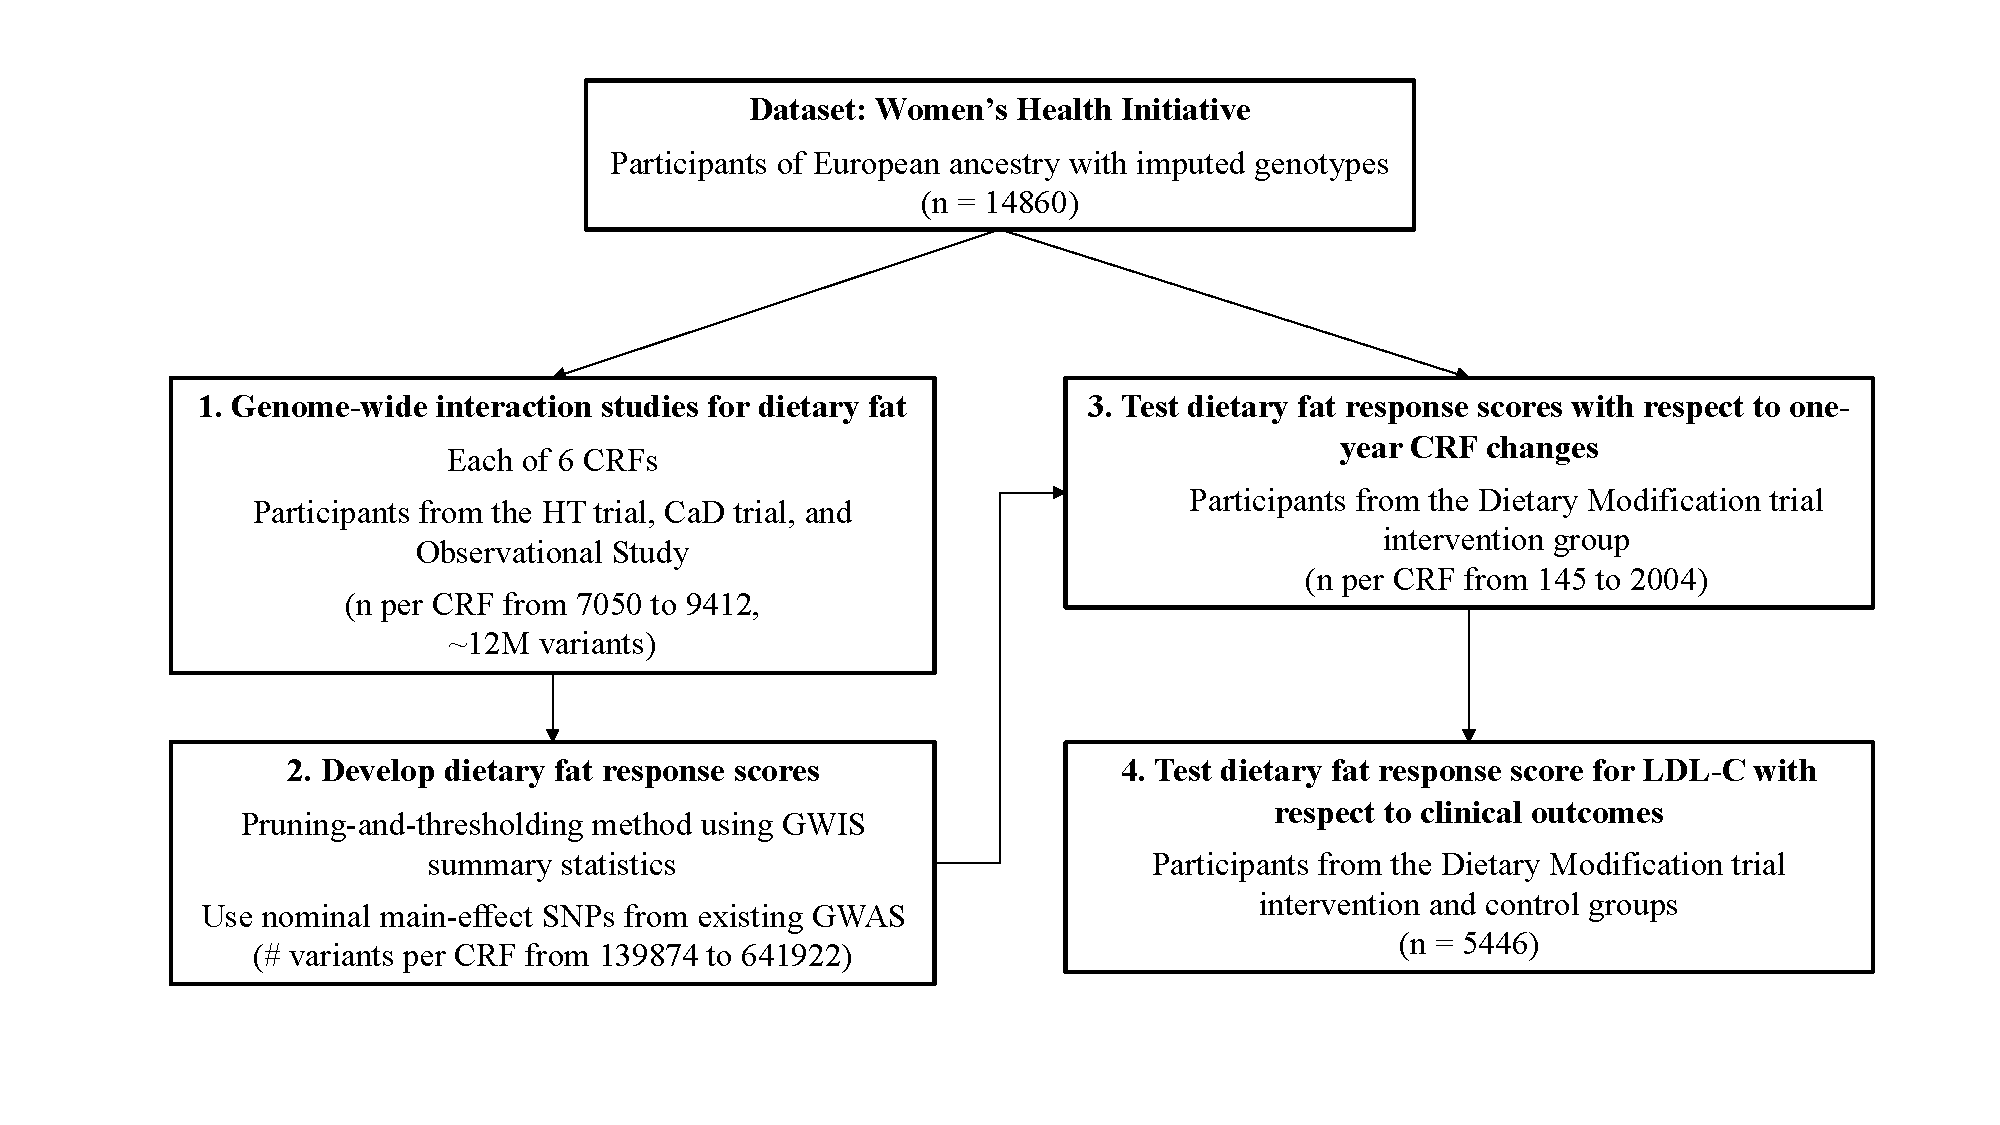
\includegraphics{workflow.pdf}
\caption{Study workflow. First, a series of genome-wide interaction
studies (GWIS) were conducted with dietary fat as the exposure for each
of six cardiovascular risk factors (CRFs). Next, dietary fat response
scores were developed using GWIS summary statistics and tested for the
prediction of one-year CRF changes in the Dietary Modification trial
intervention (with sensitivity models using the control group). Finally,
the LDL-C score was tested for the prediction of differential effects on
chronic disease development in the intervention and control groups over
approximately 22 years of follow-up. CRF: cardiometabolic risk factor,
FFQ: food frequency questionnaire, GWIS: genome-wide interaction study.}
\end{figure}

The study workflow is outlined in Figure 1. A series of genome-wide
interaction studies (GWIS) were undertaken in cross-sectional data from
the Women's Health Initiative. These GWIS incorporated only women who
did not participate in the dietary modification (DM) trial, using
imputed genotypes along with baseline self-reported dietary intakes
(from food frequency questionnaires) and fasting blood biomarkers.
Baseline characteristics of these women, along with those participating
in the DM trial, are shown in Table 1. While there were differences
across groups in almost all characteristics, they were modest in size.

\begin{ThreePartTable}
\begin{TableNotes}
\item * Continuous values shown as: median (interquartile range)
\item DM: dietary modification trial; Non-DM: all women not participating in the DM trial (enrolled in at least one of: hormone therapy trial, calcium and vitamin D trial, or observational study)
\end{TableNotes}
\begin{longtable}[t]{llll}
\caption{\label{tab:pop-description}Baseline characteristics of European-ancestry participants in the Women's Health Initiative Study (n = 17304 in total)}\\
\toprule
  & DM trial\textbackslash{}n(N = 2165 (Intervention), 3281 (Control)) & Non-DM trial\textbackslash{}n(N = 9414) & P-value\\
\midrule
Age & 66 (60-70) & 68 (64-72) & \\
Current smoking & 366 (7\%) & 888 (9\%) & <0.001\\
Lipid-lowering medication & 583 (11\%) & 1277 (14\%) & <0.001\\
Hypertension medication & 2058 (38\%) & 3416 (36\%) & <0.001\\
Diabetes medication & 269 (5\%) & 498 (5\%) & 0.07\\
Body mass index (BMI; kg/m\textasciicircum{}2) & 28.9 (25.3-33.1) & 27.2 (24-31.2) & 0.37\\
Systolic blood pressure (SBP; mm Hg) & 128 (117-140) & 144 (133-156) & <0.001\\
LDL cholesterol (LDL-C; mg/dL) & 151 (128-175) & 161 (135-192) & <0.001\\
HDL cholesterol (HDL-C; mg/dL) & 49.8 (42-58) & 51 (44-60) & <0.001\\
Triglycerides (TG; mg/dL) & 138 (100-195) & 128 (92-180) & <0.001\\
Fasting glucose (FG; mg/dL) & 97 (90-108) & 97.5 (90-113.4) & <0.001\\
\bottomrule
\insertTableNotes
\end{longtable}
\end{ThreePartTable}

Preliminary power calculations were undertaken, based on parameter
assumptions including a modest SNP main effect (0.5\%) under an additive
model and a binary environment with 50\% prevalence explaining 10\% of
the outcome phenotypic variance. The results showed that, at the sample
sizes available for European ancestry non-DM participants (7050-9412
individuals for each cardiometabolic risk factor (CRF)), this analysis
was powered to detect only moderately large interaction effects (GxE
variance explained greater than approximately 0.5\%) at genome-wide
significance (Supplementary Table 1).

Dietary fat response scores were generated for each CRF using results
from the corresponding GWIS analysis (see Methods). Q-Q plots of the
GWIS results showed that genomic inflation was fairly well-controlled
(Supplementary Figure 1). For each CRF, the associated summary
statistics (corresponding to the fat-genotype interaction term
estimates) were filtered to include only those with nominal main-effect
associations in large-scale published GWAS. This filter was informed by
the power analysis above and chosen as a compromise between discovery
and statistical power (alternative results using either a more stringent
threshold or no filtering are shown in Supplementary Table 2). A
pruning-and-thresholding method was used to generate six FRS from these
individual sets of summary statistics along with genotypes from the WHI
DM participants as a linkage disequilibrium (LD) reference. Using
parameters of seed p-value=0.05 and LD
r\textsuperscript{2}\textless{}0.5, six sets of score weights were
generated, with relevant SNP set sizes ranging from 1536 (SBP) to 6042
(BMI). Scores were then calculated as the weighted sum of allele dosages
across SNPs, normalized by the number of non-missing SNPs per
individual.

\hypertarget{dietary-fat-responder-score-assessment}{%
\subsection{Dietary fat responder score
assessment}\label{dietary-fat-responder-score-assessment}}

\begin{ThreePartTable}
\begin{TableNotes}
\item[1] Baseline-adjusted models are adjusted for the baseline value of the CRF being tested
\item[2] N\_GWIS = sample size available for the associated GWIS (non-DM participants).
\item[3] N = sample size available for DM participants with 1-year follow-up measurements for the CRF in question
\item[4] Std. effect size represents the regression coefficient estimate in terms of CRF standard deviation per responder score standard deviation
\end{TableNotes}
\begin{longtable}[t]{lrrrrrrr}
\caption{\label{tab:test-scores}Responder score effects on 1-year CRF changes in DM trial participants}\\
\toprule
\multicolumn{4}{c}{ } & \multicolumn{2}{c}{Univariate} & \multicolumn{2}{c}{Baseline-adjusted\textsuperscript{1}} \\
\cmidrule(l{3pt}r{3pt}){5-6} \cmidrule(l{3pt}r{3pt}){7-8}
Risk factor & N_GWIS\textsuperscript{2} & \# SNPs in risk score & N\textsuperscript{3} & Std. effect size\textsuperscript{4} & P-value & Std. effect size\textsuperscript{4} & P-value\\
\midrule
BMI & 9358 & 6042 & 1988 & 0.03 & 0.189 & 0.03 & 0.218\\
SBP & 9412 & 1536 & 2004 & 0.03 & 0.125 & 0.04 & 0.041\\
LDL-C & 7050 & 1760 & 145 & -0.19 & 0.020 & -0.21 & 0.005\\
HDL-C & 7157 & 1731 & 150 & -0.08 & 0.320 & -0.08 & 0.351\\
TG & 7158 & 1774 & 150 & -0.15 & 0.055 & -0.14 & 0.053\\
FG & 7200 & 1924 & 281 & 0.01 & 0.853 & 0.02 & 0.689\\
\bottomrule
\insertTableNotes
\end{longtable}
\end{ThreePartTable}

As the scores were developed to predict a positive interaction with
dietary fat intake, the expected direction of the FRS effect on risk
factors in the present fat-reduction trial would be negative. Of the fat
response scores examined, only the LDL-C fat response score (LDL-FRS)
was predictive at p \textless{} 0.05 of the associated CRF change in DM
trial participants in the fat-reduction arm (passing a Bonferroni
correction for the 6 CRFs tested in baseline-adjusted sensitivity
models; results for all scores shown in Table 2). For this score, the
standardized effect size was -0.19 (corresponding to a 5.44 mg/dL
greater decrease in LDL-C per score standard deviation; p=0.02). We note
that the sample size of European-ancestry DM trial participants with
follow-up measurements was much smaller for biochemical variables
(n\textasciitilde{}150) compared to BMI and SBP
(n\textasciitilde{}2000). Using the score developed in European-ancestry
individuals, score performance was then tested in a combined-ancestry
group including Black and Hispanic individuals, which almost doubled the
sample size (Supplementary Table 3). While some traits showed strong
relationships (e.g.~SBP), the signs of many were in a counter-intuitive
direction, including a flip in sign for the previously-strong LDL-C
relationship, suggesting that these results may reflect the known
difficulties in conducting trans-ancestry polygenic prediction (due to
differences in linkage disequilibrium among other factors) rather than
the intended biological differences. This observation was reinforced by
the lack of association of the score with CRF changes in either Blacks
or Hispanics alone. Using the LDpred algorithm, which considers the full
genome-wide set of SNPs, no predictive FRS effects were detected
(Supplementary Table 4), possibly reflecting a lack of power to overcome
the multiple testing burden without a nominal main-effect filter.

Based on its observed association in European-ancestry participants, the
LDL-FRS was investigated further. Linear models showed that the LDL-FRS
accounted for 3.7\% (95\% CI: 0.09, 11.9) of the variance in 1-year
LDL-C changes in the DM intervention arm. In baseline-adjusted models,
this figure rose slightly to 4.3\%, based on the change in
R\textsuperscript{2} compared to a baseline-only model. Further
adjustment for four principal components of baseline metabolic
biomarkers (see Methods) did not materially affect this estimate
(4.5\%). For comparison, baseline LDL-C plus these four principal
components alone explained 21.7\% of this variance, although we note
that this estimate is likely biased upward due to regression to the mean
effects (arising from measurement error and stochastic biological
fluctuations) (29). Additional baseline-adjusted models confirmed an
interaction between DM trial arm and the LDL-FRS (p=0.002), supporting
the specificity of this score for the fat-reduction arm, though the
interaction directly with self-reported change in dietary fat was weaker
(p=0.11). The LDL-FRS also showed specificity for LDL-C in that it did
not predict changes in any other CRF (Supplementary Table 5). The 1760
component SNPs were annotated using Annovar (19), revealing a
predominance of intergenic and intronic variants and a set of genes with
high numbers of independent SNPs contributing to the score (Figure
2A-D). Top genes by number of contributing SNPs included \emph{CSMD1},
\emph{PTPRD}, and \emph{RGS12}.

\begin{figure}
\centering
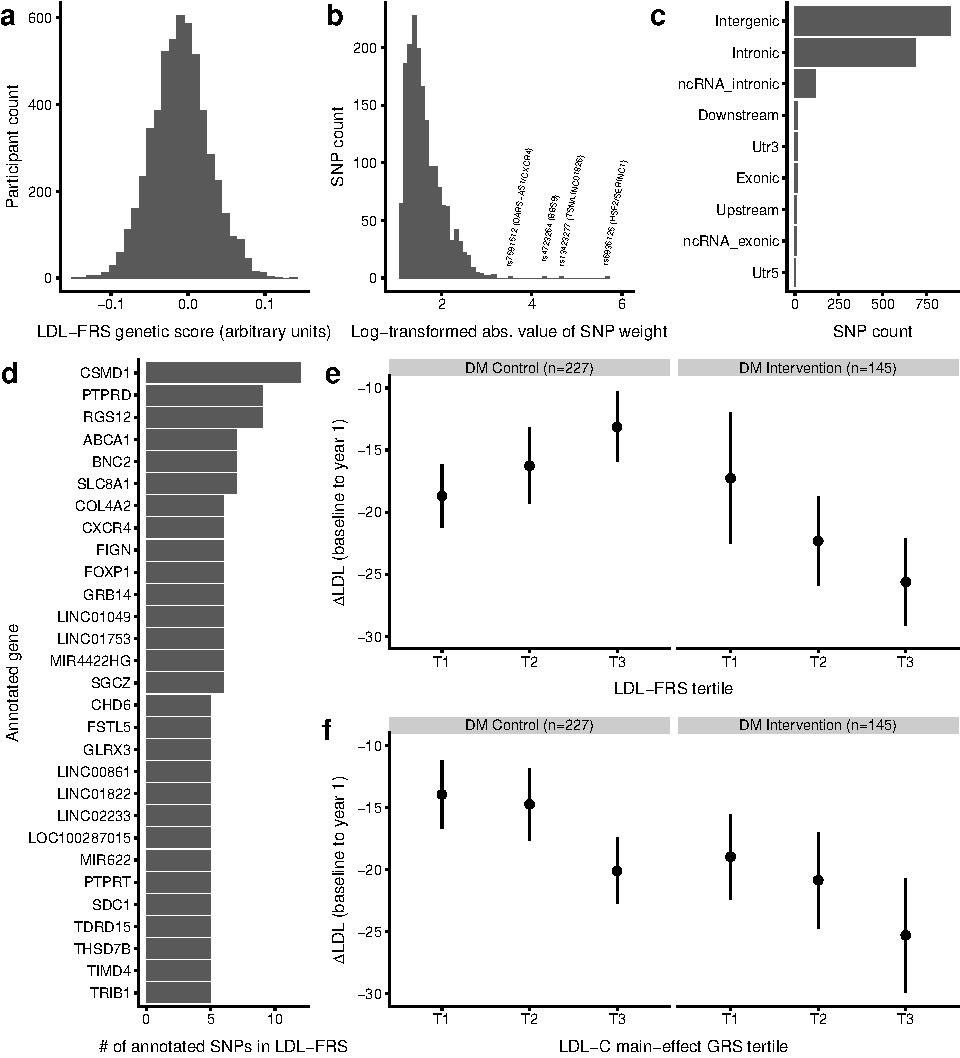
\includegraphics{figures/ldl-score-characterization-1.pdf}
\caption{LDL-FRS characterization. a) Distribution of LDL-FRS in WHI DM
trial participants. b) Distribution of SNP weights constituting the
LDL-FRS (shown as the natural log-transformed absolute values of the
true weights). c) SNP counts in different loci types for LDL-FRS
constituent SNPs. d) Genes are summarized by the number of annotated
SNPs in the LDL-FRS (genes with at least 5 component SNPs are shown).
e-f) 1-year changes in LDL-C in DM trial participants as a function of
genetic scores. Mean changes in LDL-C (y-axis) are shown as a function
of either LDL-FRS (e) or LDL-GRS (f) tertile (x-axis). Error bars
represent standard errors. LDL-FRS: LDL-C fat response genetic score,
GRS: LDL-C main-effect genetic risk score.}
\end{figure}

Differences in mean LDL-C changes during the DM trial across genetic
score strata are shown in Figure 2E,F. As suggested by the regression
results, those in the control arm trended towards less strong LDL-C
reductions in higher LDL-FRS strata, while those in the fat-reduction
arm showed the opposite trend. Furthermore, isolation of individuals at
the highest extreme of the score (top 10\%) revealed an LDL-C reduction
of almost double that of the rest of the DM intervention group (-36.4
versus -20.3 mg/dL; 95\% CI for the difference: {[}-1, 33.2{]}). For
comparison to the FRS, a main-effect genetic risk score (GRS) for LDL-C
was developed using summary statistics from the Global Lipid Genetics
Consortium meta-analysis (23) and an identical pruning-and-thresholding
procedure to that used for the FRS. As expected, this score was strongly
predictive of baseline LDL-C concentrations (p=1.45e-22). However,
unlike the FRS, the GRS did not predict LDL-C changes in the DM
intervention group (p=0.19; stratum-specific mean changes in Figure 2F).

\hypertarget{ldl-frs-association-with-chronic-disease-outcomes}{%
\subsection{LDL-FRS association with chronic disease
outcomes}\label{ldl-frs-association-with-chronic-disease-outcomes}}

\begin{figure}
\centering
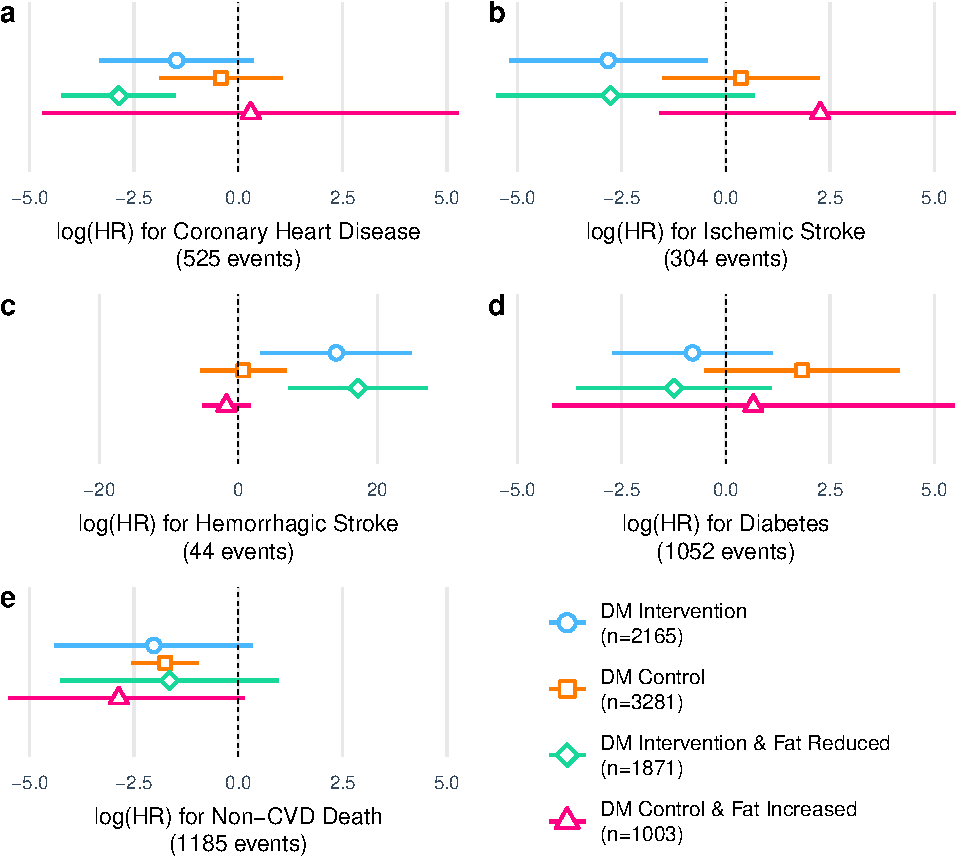
\includegraphics{figures/outcomes-1.pdf}
\caption{LDL-FRS prediction of chronic disease development. X-axis shows
log-hazard ratio estimates for the LDL-FRS from Cox proportional hazards
regression for a) coronary heart disease, b) ischemic stroke c)
hemorrhagic stroke, d) diabetes, and e) non-CVD death. Separate
estimates are shown for DM trial intervention arm, control arm, and the
same strata filtered for FFQ-reported fat reduction or increase,
respectively. Cox models are adjusted for age at baseline and include a
random effect for WHI genotyping sub-study. Error bars represent 95\%
confidence interval estimates for the regression coefficients.}
\end{figure}

Next, the LDL-FRS was tested for relationships with incident disease
outcomes over approximately 22 years of follow-up using Cox proportional
hazards models (Figure 3). The mean follow-up time for coronary heart
disease (CHD) was 8.7 years (std. dev. = 5.6), with similar values for
other outcomes. In addition to intervention versus control arm, another
set of ``per protocol-like'' strata was produced by additionally
filtering for FFQ-based self-reported fat reduction (in the intervention
group) or fat increase (in the control group). CHD qualitatively showed
the expected interaction, i.e.~a stronger inverse association between
LDL-FRS and disease risk in the fat reduction group). Ischemic stroke
showed a similar pattern, with a risk reduction only in the fat
reduction group (p = 0.029). In contrast, hemorrhagic stroke, while
having a low number of events (44 in total), showed a positive
association only in the fat reduction group (p = 0.011). Results for
diabetes qualitatively mirrored those for CHD and ischemic stroke, while
those for non-CVD death did not vary across groups. These cross-arm
differences were generally strengthened when comparing the per
protocol-like strata, with a much stronger effect for CHD in the
confirmed fat reduction stratum (p = 0.005). In DM trial arm interaction
models (score x arm), only ischemic stroke reached nominal statistical
significance (p \textless{} 0.05).

\begin{verbatim}
## Parsed with column specification:
## cols(
##   Type = col_character(),
##   Gene = col_character(),
##   CHR = col_double(),
##   POS = col_double(),
##   POS2 = col_double(),
##   REF = col_character(),
##   ALT = col_character(),
##   SNP = col_character(),
##   BETA = col_double()
## )
\end{verbatim}

\hypertarget{discussion}{%
\section{Discussion}\label{discussion}}

Diet response scores have shown some success in predicting the response
of cardiovascular risk factors (CRFs) to nutritional interventions, but
they are often based solely on main effects or single GDI SNPs. Here, we
explored the potential for genome-wide gene diet interaction (GDI)-based
diet responder score development, leveraging the multi-trial setup of
the Women's Health Initiative. We developed what to our knowledge is the
first example of a diet response score based on a hypothesis-free genome
scan for each of six risk factors, and showed preliminary evidence for
the viability of a LDL-C fat response score. The set of SNPs used for
each score were limited to those showing nominal main effects in
large-scale GWAS as a compromise between discovery and utilization of
prior information, which was supported by the weaker results in
sensitivity models incorporating either stronger (suggestive
main-effect) or weaker (all SNPs, LDpred) variant filters (Supplementary
Table 2).

Though FRS for six CRFs were developed and tested, only that for LDL-C
showed nominal significance in predicting 1-year changes in the
corresponding CRF. Multiple factors could explain this lack of
predictive performance in general. First, analysis in observational
datasets carries with it the potential for confounding of the observed
relationships. Second, FFQs are imprecise instruments for measuring
dietary intake, and though the FFQs used in the present study were
optimized for detection of dietary fat, there was potential for
substantial misclassification of this environmental exposure. Third,
power calculations shown here and elsewhere suggest that a cohort of
this size may not be powered to detect many very small gene-environment
interactions such as are sought in genome-wide approaches like the one
used here.

\emph{CSMD1}, \emph{PTPRD}, and \emph{RGS12} stood out as genes
containing the highest number of SNPs in the LDL-FRS (11, 9, and 9,
respectively, after LD-pruning for r\textsuperscript{2} \textless{} 0.5.
\emph{CSMD1} variants are notably associated with LDL-C response to
statin treatment (30) as well as SBP response to a high-salt diet (31).
\emph{CSMD1} has also shown epigenetic associations with LDL-C (32) as
well as response to modification of dietary fat composition (33).
\emph{PTPRD} variants modulate the response of T2D patients to
pioglitazone therapy (34) and show suggestive associations with eating
behaviors (caloric intake at dinner) (35). \emph{RGS12} has been linked
to LDL-C in GWAS (36). Altogether, these genes have literature evidence
for relationships to dietary intake, response to cardiometabolic
therapies, and LDL-C, but have not until now been shown to directly
modify the LDL-C response to dietary fat proportions. We note that there
is a bias towards identifying LDL-C-related variants in the LDL-FRS, as
only nominally-associated main-effect SNPs were used as input to the
score development algorithm.

A reasonable body of literature exists establishing GDIs for both
dietary fat on CRFs (37,38) and general dietary exposures on LDL-C (39).
Multiple studies have looked specifically at genetic variants modulating
the LDL-C response to dietary fat. For example, a caloric restriction
intervention in type 2 diabetics was more effective in reducing LDL-C in
ApoE4 carriers (-15.6\% versus -0.7\%) (40). In the POUNDS LOST trial,
carriers of specific alleles at APOA5 and CETP variants saw 7.5 and 8.9
mg/dL greater LDL-C decreases during a low-fat dietary intervention
(41,42). Our observed effect size of a 5.4 mg/dL decrease in LDL-C is of
a similar magnitude, and emerged despite the multi-factorial nature of
the WHI dietary intervention. The observed variance explained of 3.4\%
for the LDL-FRS means that the score, while contributing meaningfully to
the prediction, does not capture most of the interindividual variability
in LDL-C response to the WHI DM trial intervention. This explanatory
power was modestly strengthened after adjustment for baseline LDL-C as
well as principal components reflecting baseline metabolic biomarker
patterns. Based on prior observations of an inflection point in the
impact of various genetic risk scores near the 90th percentile (43), we
additionally evaluated the impact of LDL-FRS in the top 10\%, finding
almost double the LDL-C reduction in DM intervention participants with
values at this extreme.

The potential clinical utility of these findings can be evaluated in the
context of a framework recently put forth for the scientific assessment
of gene-diet interaction (44). This genetic score was developed using a
rigorous study design starting in an observational cohort an validating
in a randomized trial, and relies on an ``intermediate'' interaction in
which not only the dietary intervention but also multiple other
biological factors are expected to influence LDL-C concentrations. Given
that the biological plausibility is difficult to determine for a
polygenic score and that the scientific validity of this FRS x diet
interaction would be classified as ``possible'' to ``probable'',
additional validation of this or similar scores would be needed to
render it clinically actionable.

There has been interest in the past in using main-effect genetic risk
scores (GRS) as genetic variables in order to improve statistical power
to detect gene-environment interactions (45). Such interactions may be
viewed from a lens in which genetic risk corresponds to a predisposition
that is only triggered in certain environments (e.g.~dietary behaviors).
Here, we observed only a minor association of a main-effect GRS for
LDL-C with greater LDL-C reductions in the DM trial (p=1.9e-01). This
trend runs counter to a prior observation of greater lifestyle
intervention effectiveness for LDL-C reduction in those with low genetic
risk of hyperlipidemia (46). This discrepancy may be due to differences
between the DM trial and the personalized diet and lifestyle changes
recommended in the intervention in question. Regardless, the meaningful
increase in predictive power of the FRS compared to the main-effect GRS
for LDL-C indicates the value in using interaction-based scores rather
than simple genetic predispositions for the development of personalized
dietary recommendations.

A useful diet response score should also predict downstream changes in
chronic disease risk. Suggestive interactions for CHD, ischemic stroke,
and diabetes were apparent across strata (Figure 3A,B,D), corresponding
to a decreased risk in fat-reduction participants (whose LDL-C would be
expected to drop more prominently according to the score). In contrast,
hemorrhagic stroke showed the opposite trend, with a positive
score-disease relationship only in the fat reduction group. This result
is in line with existing evidence for the detrimental effects of low
LDL-C on hemorrhagic stroke risk (47). Non-CVD death showed no major
associations, which could be expected due to the dominance of this
category by cancer outcomes and the equivocal associations of cancer
with lipids (48). We note that all disease outcome relationships
assessed here are subject to the major caveat that dietary evolution and
decreased adherence likely developed over time in many subjects,
diluting the utility of the randomization and 1-year changes used for
stratification in Figure 3.

The present study had the advantage of developing a diet-focused genetic
score in almost 10,000 women and testing in a dietary intervention trial
using independent individuals from the same population. However, nominal
main-effect SNPs were prioritized to improve statistical power given
this moderate sample size, an approach which may fail to identify
interactions with effect directions opposite that of the main effect.
Smaller fractions of alternate ancestries in this population also made
development of ancestry-specific response scores unrealistic.
Additionally, the DM trial intervention in which the scores were tested
may not exactly match the intervention relevant to the purely fat
reduction-focused score developed here; it included additional
non-fat-related dietary recommendations that may have affected the
interactions examined here, and did not ultimately achieve its intended
20\% fat reduction. Finally, this study only examined women, despite the
fact that CRF profiles and their genetic trait architectures are known
to vary across sexes (49).

In summary, we present a method for the development of diet response
scores based on genome-wide, observational gene-diet interaction study
summary statistics. We provide proof-of-concept that a genetic score
focused on LDL-C may be useful for predicting changes in both
cardiometabolic risk factors and long-term disease risk during a dietary
intervention. However, not all dietary fat response scores derived here
were informative, highlighting the continued need for increased sample
sizes and improved diet measures for the discovery of sufficiently
robust genetic interactions genome-wide. Our results provide a
foundation for future investigations using new datasets and dietary
variables to explore the genetic architecture of diet response.

\hypertarget{acknowledgements}{%
\section{Acknowledgements}\label{acknowledgements}}

\hypertarget{conflicts-of-interest}{%
\subsection{Conflicts of Interest}\label{conflicts-of-interest}}

The authors have no conflicts of interest to disclose.

\hypertarget{authors-contributions}{%
\subsection{Authors' Contributions}\label{authors-contributions}}

KW and JO designed the research; KW conducted the research and performed
the statistical analysis; QL, SL, PS, PJ, DD, and JO advised the
development of the analysis; KW wrote the manuscript; QL, SL, PS, PK,
DD, and JO provided substantive review of the manuscript; JO had primary
responsibility for final content. All authors read and approved the
manuscript.

\hypertarget{references}{%
\section*{References}\label{references}}
\addcontentsline{toc}{section}{References}

\hypertarget{refs}{}
\leavevmode\hypertarget{ref-Ma2011}{}%
1. Ma Q, Lu AYH. Pharmacogenetics, Pharmacogenomics, and Individualized
Medicine. Pharmacological Reviews. 2011;63:437--59.

\leavevmode\hypertarget{ref-Corella2013}{}%
2. Corella D, Carrasco P, Sorli JV, Estruch R, Rico-Sanz J,
Martinez-Gonzalez MA, Salas-Salvado J, Covas MI, Coltell O, Aros F, et
al. Mediterranean Diet Reduces the Adverse Effect of the
TCF7L2-rs7903146 Polymorphism on Cardiovascular Risk Factors and Stroke
Incidence: A randomized controlled trial in a high-cardiovascular-risk
population. Diabetes Care. 2013;36:3803--11.

\leavevmode\hypertarget{ref-Huang2015}{}%
3. Huang T, Huang J, Qi Q, Li Y, Bray GA, Rood J, Sacks FM, Qi L. PCSK7
Genotype Modifies Effect of a Weight-Loss Diet on 2-Year Changes of
Insulin Resistance: The POUNDS LOST Trial. Diabetes Care.
2015;38:439--44.

\leavevmode\hypertarget{ref-Ordovas2018}{}%
4. Ordovas JM, Ferguson LR, Tai ES, Mathers JC. Personalised nutrition
and health. BMJ. 2018;bmj.k2173.

\leavevmode\hypertarget{ref-Corella2009}{}%
5. Corella D. APOA2, Dietary Fat, and Body Mass Index. Archives of
Internal Medicine. 2009;169:1897.

\leavevmode\hypertarget{ref-Cuda2011}{}%
6. Cuda C, Badawi A, Karmali M, El-Sohemy A. Polymorphisms in Toll-like
receptor 4 are associated with factors of the metabolic syndrome and
modify the association between dietary saturated fat and fasting
high-density lipoprotein cholesterol. Metabolism. 2011;60:1131--5.

\leavevmode\hypertarget{ref-Cornelis2006}{}%
7. Cornelis MC, El-Sohemy A, Kabagambe EK, Campos H. Coffee, CYP1A2
Genotype, and Risk of Myocardial Infarction. JAMA. 2006;295:1135.

\leavevmode\hypertarget{ref-Qi2012}{}%
8. Qi Q, Chu AY, Kang JH, Jensen MK, Curhan GC, Pasquale LR, Ridker PM,
Hunter DJ, Willett WC, Rimm EB, et al. Sugar-Sweetened Beverages and
Genetic Risk of Obesity. New England Journal of Medicine.
2012;367:1387--96.

\leavevmode\hypertarget{ref-Olsen2016}{}%
9. Olsen NJ, Ängquist L, Larsen SC, Linneberg A, Skaaby T, Husemoen LLN,
Toft U, Tjønneland A, Halkjær J, Hansen T, et al. Interactions between
genetic variants associated with adiposity traits and soft drinks in
relation to longitudinal changes in body weight and waist circumference.
The American Journal of Clinical Nutrition. 2016;104:816--26.

\leavevmode\hypertarget{ref-Smith2018}{}%
10. Smith CE, Follis JL, Dashti HS, Tanaka T, Graff M, Fretts AM,
Kilpeläinen TO, Wojczynski MK, Richardson K, Nalls MA, et al.
Genome-Wide Interactions with Dairy Intake for Body Mass Index in Adults
of European Descent. Molecular Nutrition \& Food Research.
2018;62:1700347.

\leavevmode\hypertarget{ref-Figueiredo2014}{}%
11. Figueiredo JC, Hsu L, Hutter CM, Lin Y, Campbell PT, Baron JA,
Berndt SI, Jiao S, Casey G, Fortini B, et al. Genome-Wide Diet-Gene
Interaction Analyses for Risk of Colorectal Cancer. Amos CI, editor.
PLoS Genetics. 2014;10:e1004228.

\leavevmode\hypertarget{ref-Dempfle2008}{}%
12. Dempfle A, Scherag A, Hein R, Beckmann L, Chang-Claude J, Schäfer H.
Gene--environment interactions for complex traits: definitions,
methodological requirements and challenges. European Journal of Human
Genetics. 2008;16:1164--72.

\leavevmode\hypertarget{ref-Anderson1998}{}%
13. Anderson GL, Cummings SR, Freedman LS, Furberg C, Henderson MM,
Johnson SR, Kuller LH, Manson JE, Oberman A, Prentice RL, et al. Design
of the Women's Health Initiative Clinical Trial and Observational Study.
Controlled Clinical Trials. 1998;19:61--109.

\leavevmode\hypertarget{ref-Ritenbaugh2003}{}%
14. Ritenbaugh C, Patterson RE, Chlebowski RT, Caan B, Fels-Tinker L,
Howard B, Ockene J. The women's health initiative dietary modification
trial: overview and baseline characteristics of participants. Annals of
Epidemiology. 2003;13:S87--97.

\leavevmode\hypertarget{ref-Patterson1999}{}%
15. Patterson RE, Kristal AR, Tinker LF, Carter RA, Bolton MP,
Agurs-Collins T. Measurement Characteristics of the Women's Health
Initiative Food Frequency Questionnaire. Annals of Epidemiology.
1999;9:178--87.

\leavevmode\hypertarget{ref-Rao2017}{}%
16. Rao DC, Sung YJ, Winkler TW, Schwander K, Borecki I, Cupples LA,
Gauderman WJ, Rice K, Munroe PB, Psaty BM. Multiancestry Study of
Gene--Lifestyle Interactions for Cardiovascular Traits in 610 475
Individuals From 124 Cohorts. Circulation: Cardiovascular Genetics.
2017;10:e001649.

\leavevmode\hypertarget{ref-RCoreTeam2017}{}%
17. R Core Team. R: A language and environment for statistical
computing. {[}Internet{]}. Vienna, Austria: R Foundation for Statistical
Computing; 2017. Available from: \url{https://www.r-project.org/}

\leavevmode\hypertarget{ref-Chang2015}{}%
18. Chang CC, Chow CC, Tellier LC, Vattikuti S, Purcell SM, Lee JJ.
Second-generation PLINK: rising to the challenge of larger and richer
datasets. GigaScience. 2015;4:7.

\leavevmode\hypertarget{ref-Wang2010}{}%
19. Wang K, Li M, Hakonarson H. ANNOVAR: functional annotation of
genetic variants from high-throughput sequencing data. Nucleic Acids
Research. 2010;38:e164--4.

\leavevmode\hypertarget{ref-Gauderman2002}{}%
20. Gauderman WJ. Sample Size Requirements for Association Studies of
Gene-Gene Interaction. American Journal of Epidemiology.
2002;155:478--84.

\leavevmode\hypertarget{ref-Yengo2018}{}%
21. Yengo L, Sidorenko J, Kemper KE, Zheng Z, Wood AR, Weedon MN,
Frayling TM, Hirschhorn J, Yang J, Visscher PM. Meta-analysis of
genome-wide association studies for height and body mass index in 700000
individuals of European ancestry. Human Molecular Genetics.
2018;27:3641--9.

\leavevmode\hypertarget{ref-Ehret2011}{}%
22. Ehret GB, Munroe PB, Rice KM, Bochud M, Johnson AD, Chasman DI,
Smith AV, Tobin MD, Verwoert GC, Hwang SJ, et al. Genetic variants in
novel pathways influence blood pressure and cardiovascular disease risk.
Nature. 2011;478:103--9.

\leavevmode\hypertarget{ref-Willer2013}{}%
23. Willer CJ, Schmidt EM, Sengupta S, Peloso GM, Gustafsson S, Kanoni
S, Ganna A, Chen J, Buchkovich ML, Mora S, et al. Discovery and
refinement of loci associated with lipid levels. Nature Genetics.
2013;45:1274--83.

\leavevmode\hypertarget{ref-Dupuis2010}{}%
24. Dupuis J, Langenberg C, Prokopenko I, Saxena R, Soranzo N, Jackson
AU, Wheeler E, Glazer NL, Bouatia-Naji N, Gloyn AL, et al. New genetic
loci implicated in fasting glucose homeostasis and their impact on type
2 diabetes risk. Nature Genetics. 2010;42:105--16.

\leavevmode\hypertarget{ref-Cha2018}{}%
25. Cha S, Kang J, Lee J-H, Kim J, Kim H, Yang Y, Park W-Y, Kim J.
Impact of Genetic Variants on the Individual Potential for Body Fat
Loss. Nutrients. 2018;10:266.

\leavevmode\hypertarget{ref-Vilhjalmsson2015}{}%
26. Vilhjálmsson BJ, Yang J, Finucane HK, Gusev A, Lindström S, Ripke S,
Genovese G, Loh P-R, Bhatia G, Do R, et al. Modeling Linkage
Disequilibrium Increases Accuracy of Polygenic Risk Scores. The American
Journal of Human Genetics. 2015;97:576--92.

\leavevmode\hypertarget{ref-ODonovan2015}{}%
27. O'Donovan CB, Walsh MC, Nugent AP, McNulty B, Walton J, Flynn A,
Gibney MJ, Gibney ER, Brennan L. Use of metabotyping for the delivery of
personalised nutrition. Molecular Nutrition \& Food Research.
2015;59:377--85.

\leavevmode\hypertarget{ref-Munda2014}{}%
28. Munda M, Legrand C. Adjusting for centre heterogeneity in
multicentre clinical trials with a time-to-event outcome. Pharmaceutical
Statistics. 2014;13:145--52.

\leavevmode\hypertarget{ref-Barnett2005}{}%
29. Barnett AG, Pols JC van der, Dobson AJ. Regression to the mean: what
it is and how to deal with it. International Journal of Epidemiology.
2005;34:215--20.

\leavevmode\hypertarget{ref-Thompson2009}{}%
30. Thompson JF, Hyde CL, Wood LS, Paciga SA, Hinds DA, Cox DR, Hovingh
GK, Kastelein JJ. Comprehensive Whole-Genome and Candidate Gene Analysis
for Response to Statin Therapy in the Treating to New Targets (TNT)
Cohort. Circulation: Cardiovascular Genetics. 2009;2:173--81.

\leavevmode\hypertarget{ref-Newton-Cheh2009}{}%
31. Newton-Cheh C, Johnson T, Gateva V, Tobin MD, Bochud M, Coin L,
Najjar SS, Zhao JH, Heath SC, Eyheramendy S, et al. Genome-wide
association study identifies eight loci associated with blood pressure.
Nature Genetics. 2009;41:666--76.

\leavevmode\hypertarget{ref-Bell2012}{}%
32. Bell JT, Tsai P-C, Yang T-P, Pidsley R, Nisbet J, Glass D, Mangino
M, Zhai G, Zhang F, Valdes A, et al. Epigenome-Wide Scans Identify
Differentially Methylated Regions for Age and Age-Related Phenotypes in
a Healthy Ageing Population. Li J, editor. PLoS Genetics.
2012;8:e1002629.

\leavevmode\hypertarget{ref-Perfilyev2017}{}%
33. Perfilyev A, Dahlman I, Gillberg L, Rosqvist F, Iggman D, Volkov P,
Nilsson E, Risérus U, Ling C. Impact of polyunsaturated and saturated
fat overfeeding on the DNA-methylation pattern in human adipose tissue:
a randomized controlled trial. The American Journal of Clinical
Nutrition. American Society for Nutrition; 2017;105:991--1000.

\leavevmode\hypertarget{ref-Pei2013}{}%
34. Pei Q, Huang Q, Yang G-p, Zhao Y-c, Yin J-y, Song M, Zheng Y, Mo
Z-h, Zhou H-h, Liu Z-q. PPAR-\(\gamma\)2 and PTPRD gene polymorphisms
influence type 2 diabetes patients' response to pioglitazone in China.
Acta Pharmacologica Sinica. 2013;34:255--61.

\leavevmode\hypertarget{ref-Comuzzie2012}{}%
35. Comuzzie AG, Cole SA, Laston SL, Voruganti VS, Haack K, Gibbs RA,
Butte NF. Novel Genetic Loci Identified for the Pathophysiology of
Childhood Obesity in the Hispanic Population. Crawford DC, editor. PLoS
ONE. 2012;7:e51954.

\leavevmode\hypertarget{ref-Spracklen2017}{}%
36. Spracklen CN, Chen P, Kim YJ, Wang X, Cai H, Li S, Long J, Wu Y,
Wang YX, Takeuchi F, et al. Association analyses of East Asian
individuals and trans-ancestry analyses with European individuals reveal
new loci associated with cholesterol and triglyceride levels. Human
Molecular Genetics. 2017;26:1770--84.

\leavevmode\hypertarget{ref-Cuda2012}{}%
37. Badawi A, Cuda, Garcia-Bailo, Karmali, El-Sohemy. A common
polymorphism near the interleukin-6 gene modifies the association
between dietary fat intake and insulin sensitivity. Journal of
Inflammation Research. 2012;1.

\leavevmode\hypertarget{ref-Zheng2015}{}%
38. Zheng Y, Huang T, Zhang X, Rood J, Bray GA, Sacks FM, Qi L. Dietary
Fat Modifies the Effects of FTO Genotype on Changes in Insulin
Sensitivity. The Journal of Nutrition. 2015;145:977--82.

\leavevmode\hypertarget{ref-Ordovas2011}{}%
39. Ordovás JM, Robertson R, Cléirigh EN. Gene--gene and
gene--environment interactions defining lipid-related traits. Current
Opinion in Lipidology. 2011;22:129--36.

\leavevmode\hypertarget{ref-Saito2004}{}%
40. Saito M, Eto M, Nitta H, Kanda Y, Shigeto M, Nakayama K, Tawaramoto
K, Kawasaki F, Kamei S, Kohara K, et al. Effect of Apolipoprotein E4
Allele on Plasma LDL Cholesterol Response to Diet Therapy in Type 2
Diabetic Patients. Diabetes Care. 2004;27:1276--80.

\leavevmode\hypertarget{ref-Zhang2012}{}%
41. Zhang X, Qi Q, Bray GA, Hu FB, Sacks FM, Qi L. APOA5 genotype
modulates 2-y changes in lipid profile in response to weight-loss diet
intervention: the Pounds Lost Trial. The American Journal of Clinical
Nutrition. 2012;96:917--22.

\leavevmode\hypertarget{ref-Xu2015}{}%
42. Xu M, Ng SS, Bray GA, Ryan DH, Sacks FM, Ning G, Qi L. Dietary Fat
Intake Modifies the Effect of a Common Variant in the LIPC Gene on
Changes in Serum Lipid Concentrations during a Long-Term Weight-Loss
Intervention Trial. The Journal of Nutrition. 2015;145:1289--94.

\leavevmode\hypertarget{ref-Khera2018}{}%
43. Khera AV, Chaffin M, Aragam KG, Haas ME, Roselli C, Choi SH,
Natarajan P, Lander ES, Lubitz SA, Ellinor PT, et al. Genome-wide
polygenic scores for common diseases identify individuals with risk
equivalent to monogenic mutations. Nature Genetics. 2018;50:1219--24.

\leavevmode\hypertarget{ref-Grimaldi2017}{}%
44. Grimaldi KA, Ommen B van, Ordovas JM, Parnell LD, Mathers JC, Bendik
I, Brennan L, Celis-Morales C, Cirillo E, Daniel H, et al. Proposed
guidelines to evaluate scientific validity and evidence for
genotype-based dietary advice. Genes \& Nutrition. 2017;12:35.

\leavevmode\hypertarget{ref-Aschard2016}{}%
45. Aschard H. A perspective on interaction effects in genetic
association studies. Genetic Epidemiology. 2016;40:678--88.

\leavevmode\hypertarget{ref-Zubair2019}{}%
46. Zubair N, Conomos MP, Hood L, Omenn GS, Price ND, Spring BJ, Magis
AT, Lovejoy JC. Genetic Predisposition Impacts Clinical Changes in a
Lifestyle Coaching Program. Scientific Reports. 2019;9:6805.

\leavevmode\hypertarget{ref-Sun2019a}{}%
47. Sun L, Clarke R, Bennett D, Guo Y, Walters RG, Hill M, Parish S,
Millwood IY, Bian Z, Chen Y, et al. Causal associations of blood lipids
with risk of ischemic stroke and intracerebral hemorrhage in Chinese
adults. Nature Medicine. 2019;25:569--74.

\leavevmode\hypertarget{ref-Koene2016}{}%
48. Koene RJ, Prizment AE, Blaes A, Konety SH. Shared Risk Factors in
Cardiovascular Disease and Cancer. Circulation. 2016;133:1104--14.

\leavevmode\hypertarget{ref-Knopp2006}{}%
49. Knopp RH, Paramsothy P, Retzlaff BM, Fish B, Walden C, Dowdy A,
Tsunehara C, Aikawa K, Cheung MC. Sex differences in lipoprotein
metabolism and dietary response: Basis in hormonal differences and
implications for cardiovascular disease. Current Cardiology Reports.
2006;8:452--9.


\end{document}
